%!TEX root = IntroArithGrps.tex

\mychapter{What is a\texorpdfstring{\\}{ }Locally Symmetric Space?}
\label{WhatisLocSymmChap}

\prereqs{understanding of geodesics, and other concepts of Differential Geometry.}

In this chapter, we give a geometric introduction to the notion of a
symmetric space or a locally symmetric space, and explain the
central role played by simple Lie groups and their lattice subgroups.
(Since geometers are the target audience here, we assume familiarity with differential geometry that will not be needed in other parts of the book.)
This material is not a prerequisite for reading any of the later
chapters, except \cref{GeomIntroRank}; it is intended to provide
a geometric motivation for the study of lattices in semisimple Lie
groups. Since arithmetic subgroups are the primary examples of lattices, this also motivates the main topic of the rest of the book.




%\section{A quick review of Riemannian manifolds and their geodesics}
%
%\begin{defn}
% Let $M$ be a topological space.
% An ($n$-dimensional) \defit{coordinate system} on an open set~$U$
%of~$M$ is a diffeomorphism~$\phi$ from~$U$ onto an open subset
%of~$\real^n$. An ($n$-dimensional) \defit[atlas on a
%manifold]{atlas} on~$M$ is a collection $\{(\phi_\alpha,
%U_\alpha)\}_{\alpha \in A}$ of $n$-dimensional coordinate
%systems on~$M$, for some~$n$, such that
% \begin{itemize}
% \item the coordinate patches cover~$M$ (that is,
%$\bigcup_{\alpha \in A} U_\alpha = M$), and
% \item the overlap maps are diffeomorphisms (that is, for all
%$\alpha, \beta \in A$, the composition $\phi_\alpha \circ
%\phi_\beta^{-1}$ is a diffeomorphism from $\phi_\beta(U_\alpha \cap
%U_\beta)$ onto $\phi_\alpha(U_\alpha \cap U_\beta)$).
% \end{itemize}
% A (smooth) \defit{manifold} is a Hausdorff topological space~$M$,
%together with an atlas.
% \end{defn}
%
%\begin{defn}
% \ 
% \begin{itemize}
% \item An \defit{inner product} on a real vector space~$V$ is
%a symmetric, positive-definite, bilinear form $\langle \cdot
%\mid \cdot \rangle$ on~$V$. 
% \item A \defit{Riemannian manifold} is
%a smooth manifold~$M$, together with the choice of an inner
%product $\langle \cdot \mid \cdot \rangle_x$ on the tangent
%space~$T_x M$, for each $x \in M$, such that $\langle \cdot
%\mid \cdot \rangle_x$ varies smoothly as $x$ varies.
% \item The \defit[norm of a tangent vector]{norm} $\|v\|_x$ of
%a vector $v \in T_x M$ is $\sqrt{\langle v \mid v \rangle_x}$.
% \end{itemize}
% \end{defn}
%
%\begin{defn}
% If $M_1$ and~$M_2$ are Riemannian manifolds, then the
%\defit[cartesian product of Riemannian manifolds]{cartesian
%product} $M_1 \times M_2$ is also a Riemannian manifold, with
%inner product given by
% $$ \bigl\langle (u_1,u_2) \mid (v_1,v_2) \bigr\rangle_{(p_1,p_2)}
% = \langle u_1 \mid v_1 \rangle_{p_1}
% + \langle u_2 \mid v_2 \rangle_{p_2}
% $$
% for $p_i \in M_i$ and $u_i,v_i \in T_{p_i} M_i$.
% \end{defn}
%
%
%\begin{defn}
% \ 
% \begin{itemize}
% \item For any smooth curve $c \colon [a,b] \to M$ in a
%Riemannian manifold~$M$, we define the \defit[length (smooth
%curve)]{length} of~$c$ to be
% $$ \int_a^b \| c'(t)\|_{c(t)} \, dt .$$
% \item Then a topological metric~$d$ is defined on~$M$ by
% $$ d(x,y) = \inf \{\, \operatorname{length}(c) \mid
% \mbox{$c$ is a smooth curve from~$x$ to~$y$} \,\} .$$
% \item A smooth curve $\gamma \colon [a,b] \to M$ is a
%\emph{length-minimizing geodesic} if
%$\|\gamma'(t)\|_{\gamma(t)}$ is constant (independent of~$t$)
%and 
% $ \operatorname{length}(\gamma) = d \bigl( \gamma(a),
%\gamma(b) \bigr)$.
% \item A smooth curve $\gamma \colon I \to M$ is a
%\emph{geodesic} if $I$ can be written as a (locally finite)
%union of closed intervals $I_m$, such that the restriction
%$\gamma|_{I_m}$ is a length-minimizing geodesic, for each~$m$.
% \item A diffeomorphism $f \colon M_1 \to M_2$ between two
%Riemannian manifolds is an \defit{Riemannian isometry} if
%$\|Df(p)v\|_{f(v)} = \|v\|_p$, for every $(p,v) \in TM_1$. (Note
%that $f$~must also be an isometry with respect to the
%associated topological metrics on~$M_1$ and~$M_2$.)
% \end{itemize}
% \end{defn}
%
%\begin{warn}
% If $C$ is a submanifold of a Riemannian manifold~$M$, then
%$C$~is a Riemannian manifold, so there is an associated
%topological metric~$d_C$ on~$C$. There is also a metric
%$d|_C$, obtained by restricting the topological metric
%on~$M$. These two metrics can be very different, because two
%points of~$C$ that are near to each other in~$M$ may not be
%joined by a short curve that lies entirely in~$C$.
% \end{warn}
%
%\begin{prop}[(\term{Existence and Uniqueness of
%Geodesics})]\index{geodesics, existence and uniqueness}
% Let $M$ be a Riemannian manifold. For any $(p,v) \in TM$,
%there is a geodesic $\gamma \colon (-\epsilon,\epsilon) \to
%M$, for some $\epsilon > 0$, such that $\gamma(0) = p$ and
%$\gamma'(0) = v$.
%
%Furthermore, if $\overline{\gamma} \colon I \to
%M$, is any geodesic, such that $\overline{\gamma}(0) = p$ and
%$\overline{\gamma}'(0) = v$, then $\overline{\gamma}(t) = \gamma(t)$
%for all $t \in I \cap (-\epsilon,\epsilon)$.
% \end{prop}
%
% \begin{defn}
% A neighborhood~$V$ of~$0$ in a real vector space is:
% \begin{itemize}
% \item \defit{star-shaped} if $t V \subseteq V$ for all $t \in
%[0,1]$,
% \item \defit[symmetric!neighborhood]{symmetric} if $-V = V$.
% \end{itemize}
% \end{defn}
%
%\begin{cor} \label{explcoords}
% For each each $p \in M$, there is a star-shaped, symmetric
%neighborhood $V$ of~$0$ in $T_p(M)$, such that we may define a smooth
%map $\exp_p \colon V \to M$ by letting $\exp_p(v) = \gamma(1)$, where
%$\gamma$ is a geodesic such that $\gamma(0) = p$ and $\gamma'(0) = v$.
%Furthermore, if $V$ is sufficiently small, then $\exp_p$ is a
%diffeomorphism onto its image.
% \end{cor}
%
%\begin{defn}
% Note that, by identifying $T_p M$ with $\real^n$, the inverse of
%$\exp_p$ defines a coordinate system on a neighborhood of~$p$. These
%are called \defit{exponential coordinates} at~$p$.
% \end{defn}
%
%There are two different definitions of completeness for a
%Riemannian manifold. Fortunately, they are equivalent.
%
%\begin{defn}
% Let $M$ be a Riemannian manifold.
% \begin{itemize}
% \item $M$ is \defit{geodesically complete} if, for every
%geodesic segment  $\gamma \colon (-\epsilon,\epsilon) \to M$,
%there is a geodesic $\overline{\gamma} \colon \real \to M$,
%such that $\overline{\gamma}(t) = \gamma(t)$, for all $t \in
%(-\epsilon,\epsilon)$.
% \item $M$ is \defit[complete metric space]{complete} if all
%Cauchy sequences converge.
% \end{itemize}
% \end{defn}
%
%\begin{prop}
% A Riemannian manifold is geodesically complete if and only
%if it is complete.
% \end{prop}



\section{Symmetric spaces}

Recall that a \defit{Riemannian manifold} is
a smooth manifold~$M$, together with the choice of an inner
product $\langle \cdot \mid \cdot \rangle_x$ on the tangent
space~$T_x M$, for each $x \in M$, such that $\langle \cdot
\mid \cdot \rangle_x$ varies smoothly as $x$ varies.
The nicest Riemannian manifolds are homogeneous. This means that every
point looks exactly like every other point:

\begin{defn} \label{HomogDefn}
 A Riemannian manifold~$X$ is a \defit{homogeneous space} if its
isometry group $\Isom(X)$ acts transitively. That is, for every $x,y
\in X$, there is an isometry~$\phi$ of~$X$, such that $\phi(x) = y$.
 \end{defn}

\begin{notation} \label{GoNotation}
We use \nindex{$G^\circ$ = identity component of~$G$}$G^\circ$ to denote the \term{identity component} of the group~$G$.
\end{notation}

\begin{egs}
 Here are some elementary examples of (simply connected) homogeneous
spaces.
 \begin{enumerate} \itemsep=\smallskipamount
 
 \item The round sphere $S^n 
 = \{\, x \in \real^{n+1} \mid \|x\| = 1 \,\}$. Rotations are the only
orientation-preserving isometries of~$S^n$, so we have $\Isom(S^n)^\circ =
\SO(n+1)$. Any point on~$S^n$ can be rotated to any other point, so
$S^n$ is homogeneous.

 \item Euclidean space $\real^n$. Every
orientation-preserving isometry of~$\real^n$ is a combination of a
translation and a rotation, and this implies that $\Isom(\real^n)^\circ = \SO(n) \ltimes
\real^n$. Any point in~$\real^n$ can be
translated to any other point, so $\real^n$ is homogeneous. 

 \item The hyperbolic plane $\hyperbolic^2
 = \{\, z \in \complex \mid \Im z > 0 \,\}$,
 where the inner product on $T_z \hyperbolic^2$ is given by
 $$ \langle u \mid v \rangle_{\hyperbolic^2}
 = \frac{1}{4(\Im z)^2} \, \langle u \mid v \rangle_{\real^2} .$$
 It is not difficult to show that 
 	$$  \text{$\Isom(\hyperbolic^2)^\circ$ is isomorphic to 
	$\PSL(2,\real)^\circ = \SL(2,\real)/\{\pm 1\}$,} $$
by noting that
$\SL(2,\real)$ acts on $\hyperbolic^2$ by linear-fractional
transformations $z \mapsto (az+b)/(cz+d)$, and confirming, by
calculation, that these linear-fractional transformations preserve
the hyperbolic metric.

 \item Hyperbolic space
 $\hyperbolic^n = \{\, x \in \real^n \mid x_n > 0 \,\}$,
 where the inner product on $T_x \hyperbolic^n$ is given by
 $$ \langle u \mid v \rangle_{\hyperbolic^n}
 = \frac{1}{4x_n^2} \, \langle u \mid v \rangle_{\real^n} .$$
 It is not difficult to see that $\hyperbolic^n$ is homogeneous
\csee{HnisHomog}. One can also show that that
the group $\Isom(\hyperbolic^n)^\circ$ is isomorphic to
$\SO(1,n)^\circ$ \csee{HyperModel}.
 \item A cartesian product of any combination of the above
\csee{prod->homog}.
 \end{enumerate}
 \end{egs}

\begin{defns}
 Let $\phi \colon X \to X$.
 \begin{enumerate}
 \item We say that $\phi$ is \defit[involutive
isometry]{involutive} (or that $\phi$ is an \defit{involution}) if
$\phi^2 = \Id\mk$.
 \item A \defit{fixed point} of~$\phi$ is a point $p \in X$, such that
$\phi(p) = p$.
 \item A fixed point~$p$ of~$\phi$ is \defit[isolated fixed
point]{isolated} if there is a neighborhood~$U$ of~$p$, such that $p$
is the only fixed point of~$\phi$ that is contained in~$U$.
 \end{enumerate}
 \end{defns}

Besides an isometry taking $x$ to~$y$, each of the above spaces also
has a nice involutive isometry that fixes~$x$.
 \begin{enumerate} \itemsep=\smallskipamount
 \item Define $\phi_1 \colon S^n \to S^n$ by
 $$ \phi_1(x_1,\ldots,x_{n+1}) = (-x_1,\ldots,-x_n,x_{n+1}) .$$
 Then $\phi_1$ is an isometry of~$S^n$, such that $\phi_1$ has only
two fixed points: namely, $e_{n+1}$ and~$-e_{n+1}$, where $e_{n+1} =
(0,0,\ldots,0,1)$. Therefore, $e_{n+1}$ is an isolated fixed point
of~$\phi_1$.
 \item Define $\phi_2 \colon \real^n \to \real^n$ by $\phi_2(x) =
-x$. Then $\phi_2$ is an isometry of~$\real^n$, such that $0$ is the
only fixed point of~$\phi_2$.
 \item Define $\phi_3 \colon \hyperbolic^2 \to \hyperbolic^2$ by
$\phi_3(z) = -1/z$. Then $i$ is the only fixed point of~$\phi_3$.
 \item There are involutive isometries of~$\hyperbolic^n$ that have a
unique fixed point \csee{invol(BallModel)}, but they are somewhat
difficult to describe in the upper-half-space model that we are using.
 \end{enumerate}
The existence of such an isometry is the additional condition that is
required to be a symmetric space.

\begin{defn} \label{symmDefn}
 A Riemannian manifold~$X$ is a \defit[symmetric!space]{symmetric space} if
 \begin{enumerate}
 \item $X$ is connected,
 \item \label{symmDefn-homog}
 $X$ is homogeneous, and
 \item \label{symmDefn-fp}
 there is an involutive isometry~$\phi$ of~$X$, such that $\phi$ has
at least one isolated fixed point.
 \end{enumerate}
 \end{defn}

\begin{rem}
 If $X$ is a symmetric space, then all points of~$X$ are essentially
the same, so, for each $x \in X$ (not only for \emph{some} $x \in X$),
there is an isometry~$\phi$ of~$X$, such that $\phi^2 = \Id$ and $x$
is an isolated fixed point of~$\phi$ \csee{symm->xfixed}.
Conversely, if Condition~\pref{symmDefn-fp} is replaced with this
stronger assumption, then Condition~\pref{symmDefn-homog} can be
omitted \csee{xfixed->symm}.
 \end{rem}

We constructed examples of involutive isometries of $S^n$, $\real^n$,
and~$\hyperbolic^n$ that have an isolated fixed point. The following
proposition shows that no choice was involved: the involutive
isometry with a given isolated fixed point~$p$ is unique, if it
exists. Furthermore, in the exponential coordinates at~$p$, the
involution must simply be the map $x \mapsto -x$.

\begin{prop} \label{phiunique}
 Suppose $\phi$ is an involutive isometry of a Riemmanian
manifold~$X$, and suppose $p$ is an isolated fixed point of~$\phi$.
Then
 \begin{enumerate}
 \item \label{phiunique-dphi}
 $d\phi_p = - \Id$, and
 \item \label{phiunique-phi}
 for every geodesic $\gamma$ with~$\gamma(0) = p$, we have $\phi
\bigl( \gamma(t) \bigr) = \gamma(-t)$, for all $t \in \real$.
 \end{enumerate}
 \end{prop}

\begin{proof}
 \pref{phiunique-dphi} From the Chain Rule, and the fact that $\phi(p) =
p$, we have
 $$ d(\phi^2)_p = d\phi_{\phi(p)} \circ d\phi_p = (d\phi_p)^2 .$$
 Also, because $\phi^2 = \Id$, we know that $d(\phi^2)_p = d \Id_p =
\Id$. We conclude that $(d\phi_p)^2 = \Id$; hence, the linear
transformation $d\phi_p \colon T_p X \to T_p X$ satisfies the polynomial
equation $x^2 - 1 = 0$. 

Suppose $d\phi_p \neq -\Id$. (This will lead to a contradiction.)
Since the polynomial $x^2 - 1$ has no repeated roots, we know that
$d\phi_p$ is diagonalizable. Furthermore, because $1$ and~$-1$ are
the only roots of $x^2 - 1$, we know that $1$ and~$-1$ are the only
possible eigenvalues of $d\phi_p$. Therefore, because $d\phi_p \neq -\Id$,
we conclude that $1$ is an eigenvalue; so we may choose some
nonzero $v \in T_p X$, such that $d\phi_p(v) = v$. Let $\gamma$ be the
geodesic with $\gamma(0) = p$ and $\gamma'(0) = v$. Then, because
$\phi$ is an isometry, we know that $\phi \circ \gamma$ is also a
geodesic. We have 
 $$(\phi \circ \gamma)(0) = \phi \bigl( \gamma(0) \bigr)
 = \phi(p) = p = \gamma(0) $$
 and
 $$ (\phi \circ \gamma)'(0)
 = d \phi_{\gamma(0)} \bigl( \gamma'(0) \bigr)
 = d \phi_p (v)
 = v
 = \gamma'(0) .$$
 Since every geodesic is uniquely determined by prescribing its initial
position and its initial velocity, we conclude that $\phi \circ \gamma
= \gamma$. Therefore, $\phi \bigl( \gamma(t) \bigr) = \gamma(t)$, so
$\gamma(t)$ is a fixed point of~$\phi$, for every~$t$. This
contradicts the fact that the fixed point $p = \gamma(0)$ is isolated.

\pref{phiunique-phi} Define $\overline{\gamma}(t) = \gamma(-t)$, so
$\overline{\gamma}$ is a geodesic. Because $\phi$ is an isometry, we
know that $\phi \circ \gamma$ is also a geodesic. We have
 $$(\phi \circ \gamma)(0) = \phi \bigl( \gamma(0) \bigr)
 = \phi(p) = p = \overline{\gamma}(0) $$
 and, from~\pref{phiunique-dphi},
 $$ (\phi \circ \gamma)'(0)
 = d \phi_{\gamma(0)} \bigl( \gamma'(0) \bigr)
 = -\gamma'(0)
 = \overline{\gamma}'(0) .$$
 Since a geodesic is uniquely determined by prescribing its initial
position and its initial velocity, we conclude that $\phi \circ
\gamma = \overline{\gamma}$, as desired.
 \end{proof}

\begin{defn}
 Let $M$ be a Riemannian manifold, and let $p \in M$. 
It is a basic fact of differential geometry that there is a neighborhood~$V$ of~$0$ in $T_pM$, such that the exponential map $\exp_p$ maps~$V$ diffeomorphically onto a
neighborhood~$U$ of~$p$ in~$M$. By making $V$ smaller, we may assume it is:
	\begin{itemize}
	\item \defit[symmetric!neighborhood]{symmetric} (that is, $-V = V$),
	and
	\item \defit[star-shaped neighborhood]{star-shaped} (that is, $tV \subseteq V$, for $0\le t < 1$).
	\end{itemize}
The \defit{geodesic symmetry} at~$p$ is the diffeomorphism~$\tau$ of~$U$ that is defined by
 $$ \tau \bigl( \exp_p(v) \bigr) = \exp_p(-v) ,$$
 for all $v \in V$.

In other words, for each geodesic~$\gamma$ in~$M$, such that
$\gamma(0) = p$, and for all $t \in \real\mk$, such that $t \gamma'(0)
\in V$, we have $\tau \bigl( \gamma(t) \bigr) = \gamma(-t)$.
 \end{defn}

\begin{note}
 The geodesic symmetry~$\tau$ is a local diffeomorphism, but, for
most manifolds~$M$, it is \emph{not} a local isometry
\ccf{locsymm<>geodsymm}.
 \end{note}

In this terminology, the preceding proposition shows that if an
involutive isometry~$\phi$ has a certain point~$p$ as an isolated
fixed point, then, locally, $\phi$ must agree with the geodesic
symmetry at~$p$. This has the following easy consequence, which is
the motivation for the term \defit[symmetric!space]{symmetric space}.

\begin{cor} \label{symm<>geodsymm}
 A connected Riemannian manifold~$M$ is a symmetric space if and only
if, for each $p \in M$, the geodesic symmetry at~$p$ extends to an
isometry of~$M$.
 \end{cor}


\begin{exercises}

\item \label{HnisHomog}
 Show that $\hyperbolic^n$ is homogeneous. 
 \hint{For any $t
\in \real^+$, the dilation $x \mapsto tx$ is an isometry
of~$\hyperbolic^n$. Also, for any $v \in \real^{n-1}$, the
translation $x \mapsto x + v$ is an isometry of~$\hyperbolic^n$.}

\item \label{HnBallModel}
 Let $B^n = \{\, x \in \real^n \mid \|x\| < 1 \,\}$ be the open unit
ball in~$\real^n$, equip $T_x B^n$ with the inner product
 $$ \langle u \mid v \rangle_{B^n}
 = \frac{1}{ \bigl( 1 - \|x\|^2 \bigr)^2} \, \langle u \mid v
\rangle_{\real^n} ,$$
 and let $e_n = (0,0,\ldots,0,1) \in \real^n$.
 Show that the map $\phi \colon B^n \to \hyperbolic^n$ defined by
 $$ \phi(x) = \frac{x + e_n}{\|x + e_n\|^2} - \frac{1}{2} e_n$$
 is an isometry from~$B_n$ onto~$\hyperbolic^n$. (In geometric terms,
$\phi$ is obtained by composing a translation with the inversion
centered at the south pole of~$B^n$.)

\item \label{invol(BallModel)}
 Show that $x \mapsto -x$ is an isometry of~$B^n$ (with respect to the
Riemannian metric $\langle \cdot \mid \cdot \rangle_{B^n}$ defined in \cref{HnBallModel}).

\item \label{HyperModel}
 For $u,v \in \real^{n+1}$, define
 $$ \langle u \mid v \rangle_{1,n}
 = u_0 v_0 - \sum_{j=1}^n u_j v_j .$$
 (Note that, for convenience, we start our numbering of the
coordinates at~$0$, rather than at~$1$.) Let
 $$ X_{1,n}^+ = \{\, x \in \real^{n+1} \mid \langle x \mid x
\rangle_{1,n} = 1, \ x_0 > 0 \,\} ,$$
 so $X_{1,n}^+$ is one sheet of a 2-sheeted hyperboloid. Equip $T_x
X_{1,n}^+$ with the inner product obtained by restricting $\langle
\cdot \mid \cdot \rangle_{1,n}$ to this subspace. 
 \begin{enumerate}
 \item Show that the bijection $\psi \colon B^n \to X_{1,n}^+$
defined by 
 $$ \psi(x) = \frac{1}{1 - \|x\|^2} \, (1,x) $$
 is an isometry. (Note that this implies that the restriction of
$\langle \cdot \mid \cdot \rangle_{1,n}$ to $T_x X_{1,n}^+$ is
positive definite, even though $\langle \cdot \mid \cdot
\rangle_{1,n}$ is not positive definite on all of~$\real^{n+1}$.)
 \item Show $\SO(1,n)^\circ$ acts transitively on~$X_{1,n}^+$ by
isometries.
 \end{enumerate}

\item \label{Stab(Hn)} 
 For $G = \SO(1,n)^\circ = \Isom(\hyperbolic^n)^\circ$, show there is
some $p \in \hyperbolic^n$, such that $\Stab_G(p) = \SO(n)$.
 \hint{This is easy in the hyperboloid model~$X_{1,n}^+$.}

\item \label{prod->homog}
 Show that if $X_1,X_2,\ldots,X_n$ are homogeneous spaces, then the
cartesian product $X_1 \times X_2 \times \cdots \times X_n$ is also
homogeneous.

\item Show that every homogeneous space is \defit{geodesically
complete}. That is, for every geodesic segment $\gamma \colon
(-\epsilon, \epsilon) \to X$, there is a doubly-infinite geodesic
$\overline{\gamma} \colon \real \to X$, such that
$\overline{\gamma}(t) = \gamma(t)$ for all $t \in (-\epsilon,
\epsilon)$.

\item Show that if $X_1,\ldots,X_n$ are symmetric spaces, then the
cartesian product $X_1 \times X_2 \times \cdots \times X_n$ is also a
symmetric space.

\item \label{symm->xfixed}
 Show that if $X$ is a symmetric space, then, for each $x \in X$,
there is an isometry~$\phi$ of~$X$, such that $\phi^2 = \Id$ and $x$ is
an isolated fixed point of~$\phi$.

\item \label{xfixed->symm}
 Let $X$ be a connected Riemannian manifold, and assume, for each $x
\in X$, that there is an isometry~$\phi$ of~$X$, such that $\phi^2 =
\Id$ and $x$ is an isolated fixed point of~$\phi$. Show that $X$ is
homogenous, and conclude that $X$ is a symmetric space.

\item Show that the real projective space $\real P^n$ (with the metric
that makes its universal cover a round sphere) has an involutive
isometry~$\phi$, such that $\phi$ has both an isolated fixed point,
and a fixed point that is not isolated. Is $\real P^n$ a symmetric
space?

\end{exercises}



\section{How to construct a symmetric space} \label{ConstructSymm}

In this section, we describe how Lie groups are used to construct
symmetric spaces. Let us begin by recalling the well-known
group-theoretic structure of any homogeneous space.

Suppose $X$ is a connected homogeneous space, and let $G =
\Isom(X)^\circ$. Because $\Isom(X)$ is transitive on~$X$, and $X$ is
connected, we see that $G$ is transitive on~$X$
\csee{Xconn->idcomp}, so we may identify $X$ with the coset space
$G/K$, where $K$ is the stabilizer of some point in~$X$. Note that
$K$ is compact \csee{StabCpct}.

Conversely, if $K$ is any compact subgroup of any Lie group~$G$, then
there is a $G$-invariant Riemannian metric on $G/K$
\csee{G/K->Riem}, so $G/K$ (with this metric) is a homogeneous space.
 (For
any closed subgroup~$H$ of~$G$, the group~$G$ acts transitively on
the manifold $G/H$, by diffeomorphisms. However, when $H$ is not
compact, $G$ usually does not act by isometries of any Riemannian
metric on $G/H$, so there is no reason to expect $G/H$ to be a
homogeneous space in the sense of \cref{HomogDefn}.)

 \begin{eg}  \ 
 \noprelistbreak
 \begin{enumerate}
 
 \item For $X = S^n$, we have $G = \SO(n+1)$, and we may let 
 	$$ \text{$K = \Stab_G(e_{n+1}) = \SO(n)$, \ so \ $S^n = \SO(n+1)/\SO(n)$} .$$
Note that,
letting $\sigma$ be the diagonal matrix 
 $$ \sigma = \diag(-1,-1,\ldots,-1,1) ,$$ we
have $\sigma^2 = \Id$, and
  $K = \czer_G(\sigma)$ is the centralizer of~$\sigma$ in~$G$.
  
 \item For $X = \real^n$, we have $G = \SO(n) \ltimes \real^n$, and
we may let 
	$$ \text{$K = \Stab_G(0) = \SO(n)$, \ so \ $\real^n = \bigl( \SO(n)
\ltimes \real^n)/\SO(n)$} .$$
Note that the map $\sigma \colon (k,v)
\mapsto (k,-v)$ is an automorphism of~$G$, such that $\sigma^2 =
\Id$, and 
 $$ \czer_G(\sigma) = \{\, g \in G \mid \sigma(g) = g \,\} = K .$$
 
 \item For $X = \hyperbolic^2$, we have $G \approx \SL(2,\real)$, and
we may let 
	$$ \text{$K = \Stab_G(i) \approx \SO(2)$, \ so \ 
 $\hyperbolic^2 = \SL(2,\real)/\SO(2)$} .$$
  
 \item For $X = \hyperbolic^n$, we have $G = \SO(1,n)^\circ$, and we
may take $K = \SO(n)$ \csee{Stab(Hn)}.  Note that, for
$\sigma = \diag(1,-1,-1,\ldots,-1)$, we have
$\sigma^2 = \Id$, and
  $K = \czer_G(\sigma)$.
 \end{enumerate}
 Therefore, in each of these cases, there is an automorphism~$\sigma$
of~$G$, such that $K$ is the centralizer of~$\sigma$. (In other words,
$K = \{\, k \in G \mid \sigma(k) = k \,\}$ is the set of fixed points of~$\sigma$ in~$G$.) The following
proposition shows, in general, that a slightly weaker condition makes
$G/K$ symmetric, not just homogeneous.
 \end{eg}

\begin{prop} \label{G/K->symm}
 Let
 \begin{itemize}
 \item $G$ be a connected Lie group,
 \item $K$ be a compact subgroup of~$G$, and
 \item $\sigma$ be an involutive automorphism of~$G$, such that $K$
is an open subgroup of $\czer_G(\sigma)$.
 \end{itemize}
 Then $G/K$ can be given the structure of a symmetric space, such that
the map $\tau(gK) = \sigma(g) K$ is an involutive isometry of $G/K$
with $eK$ as an isolated fixed point.
 \end{prop}

\begin{proof}
 To simplify the proof slightly, let us assume that $K = \czer_G(\sigma)$
\csee{KinC(sigma)}. 

Because $K$ is compact, we know there is a $G$-invariant Riemmanian
metric on $G/K$ \csee{G/K->Riem}. Then, because $\langle \tau
\rangle$ is finite, and normalizes~$G$, it is not difficult to see
that we may assume this metric is also $\tau$-invariant
\csee{FiniteAvgMetric}. (This conclusion can also be reached by
letting $G^+ = \langle \sigma \rangle \ltimes G$ and $K^+ = \langle
\sigma \rangle \times K$, so $K^+$ is a compact subgroup of~$G^+$,
such that $G^+/K^+ = G/K$.) Therefore, $\tau$ is an involutive isometry of
$G/K$.

Suppose $gK$ is a fixed point of~$\tau$, with $g \approx e$. Then
$\sigma(g) \in g K$, so we may write $\sigma(g) = gk$, for some $k
\in K$. Since $\sigma$ centralizes~$k$ (and $\sigma$ is an
automorphism), we have
 $$\sigma^2(g) = \sigma \bigl( \sigma(g) \bigr)
 = \sigma(gk) = \sigma(g) \, \sigma(k) 
 = (gk) (k)= g k^2 .$$
 On the other hand, we know $\sigma^2(g) = g$ (because $\sigma$ is
involutive), so we conclude that $k^2 = e$.

Since $g \approx e$, and $\sigma(e) = e$, we have $\sigma(g) \approx
g$, so $k = g^{-1} \sigma(g) \approx e$. Since $k^2 = e$, we conclude
that $k = e$. (There is a neighborhood~$U$ of~$e$ in~$G$, such that,
for every $u \in U \smallsetminus \{e\}$, we have $u^2 \neq e$.) 
Therefore $\sigma(g) = gk = ge = g$, so $g \in \czer_G(\sigma) = K$;
hence, $gK = eK$.
 \end{proof}

Conversely, for any symmetric space~$X$, there exist $G$, $K$,
and~$\sigma$ as in \cref{G/K->symm}, such that $X$ is
isometric to $G/K$ \csee{symm->G/K}. 

\begin{eg} \label{SLnSymm}
 Let $G = \SL(n,\real)$, $K = \SO(n)$, and define $\sigma(g) =
(g^{-1})^T$ (the transpose-inverse). Then $\sigma^2 = 1$ and
$\czer_G(\sigma) = K$, so the theorem implies that $G/K$ is a symmetric
space. Let us describe this space somewhat more concretely.

Recall that any real symmetric matrix~$A$ can be diagonalized
over~$\real$. In particular, all of its eigenvalues are real. If all the
eigenvalues of~$A$ are strictly positive, then we say that $A$ is
\defit[positive!definite]{positive definite}.

Let 
 $$X = \{\, A \in \SL(n,\real) \mid 
 \mbox{$A$ is symmetric and positive definite} \,\} ,$$
 and define $\alpha \colon G \times X \to X$ by 
 $\alpha(g,x) = g x g^T$. 
 Then:
 \begin{enumerate} \renewcommand{\theenumi}{\alph{enumi}}
 \item \label{SLnSymm-act}
 $\alpha$ defines an action of $G$ on~$X$; i.e., we have
$\alpha(gh,x) = \alpha \bigl( g, \alpha(h,x) \bigr)$ for all $g,h \in G$
and $x \in X$.
\item \label{SLnSymm-G/K}
This action is transitive, and we have $K = \Stab_G(\Id)$, so $X$ may be
identified with $G/K$.
 \item \label{SLnSymm-TX}
 $T_{\Id} X = 
 \{\, u \in \Mat_{n\times n}(\real) \mid 
 \mbox{$u$ is symmetric and $\trace(u) = 0$} \,\} $. (By definition,
we have $X \subseteq \SL(n,\real)$. The condition $\trace(u) = 0$ is obtained by differentiating the restriction $\det(A) = 1$.)
 \item \label{SLnSymm-<>}
 The inner product $\langle u \mid v \rangle = \trace(uv)$ on
$T_{\Id} X$ is $K$-invariant, so it may be extended to a $G$-invariant
Riemannian metric on~$X$.
 \item \label{SLnSymm-tau}
 The map $\tau \colon X \to X$, defined by $\tau(A) = A^{-1}$, is an
involutive isometry of~$X$, such that 
 $\tau \bigl( \alpha(g,x) \bigr) = \sigma(g) \, \tau(x)$ for all $g
\in G$ and $x \in X$.
 \end{enumerate}
 \end{eg}

\begin{eg}
 Other examples of symmetric spaces are:
 \begin{enumerate}
 \item $\SL(n,\complex)/\SU(n)$, and
 \item $\SO(p,q)^\circ / \bigl( \SO(p) \times \SO(q) \bigr) $.
 \end{enumerate}
 \end{eg}

These are special cases of a consequence of
\cref{G/K->symm} that will be stated after we introduce some terminology.

\begin{defns} \ 
\noprelistbreak
	\begin{enumerate}
	\item A symmetric space~$X$ is \defit[irreducible!symmetric
space]{irreducible} if its universal cover is not isometric to any
nontrivial product $X_1 \times X_2$.
	\item A Riemannian manifold is \defit[flat!manifold]{flat} if its curvature tensor is identically zero, or, equivalently, if every point in~$X$ has a neighborhood that is isometric to an open subset of the Euclidean space~$\real^n$.
	\end{enumerate}
 \end{defns}

\begin{prop} \label{noncpctsymm<>simplegrp}
 Let $G$ be a connected, noncompact, simple Lie group with finite
center. Then $G$ has a maximal compact subgroup~$K$ \textup(which
is unique up to conjugacy\textup), and $G/K$ is a simply
connected, noncompact, irreducible symmetric space.
Furthermore, $G/K$ has non-positive sectional curvature and is not flat.

Conversely, any noncompact, non-flat, irreducible symmetric space is
of the form $G/K$, where $G$ is a connected, noncompact, simple Lie
group with trivial center, and $K$ is a maximal compact subgroup
of~$G$.
 \end{prop}

\begin{rem}
 Let $K$ be a compact subgroup of a connected, simple Lie group~$G$
with finite center, such that $G/K$ is a symmetric space
\ccf{G/K->symm}. \Cref{noncpctsymm<>simplegrp} shows that if $G$ is not compact,
then $K$ must be a maximal compact subgroup of~$G$, which is
essentially unique. 

On the other hand, if $G$ is compact, then the subgroup~$K$ may not
be unique, and may not be maximal. For example, both
$\SO(n)/\SO(n-1)$ and $\SO(n)/\{e\}$ are symmetric spaces. The former
is a round sphere, which has already been mentioned. The latter is a
special case of the fact that every connected, compact Lie group is a
symmetric space \csee{X=G}.

\'E.\,Cartan obtained a complete list of all the symmetric spaces
(both compact and noncompact) by finding all of the simple Lie
groups~$G$ \csee{RealSimpleGrps}, and determining, for each of them, which compact subgroups~$K$ can arise in
\cref{G/K->symm}.
 \end{rem}

\begin{exercises}

\item \label{Xconn->idcomp}
 Suppose a topological group~$G$ acts transitively (and continuously)
on a connected topological space~$M$. Show that the identity component
$G^\circ$ is transitive on~$M$.

\item \label{StabCpct}
 Let $\{g_n\}$ be a sequence of isometries of a connected, complete Riemannian manifold~$M$, and assume there exists $p \in M$, such that $g_n p = p$ for all~$n$.) Show there is a subsequence $\{g_{n_k}\}$ of~$\{g_n\}$ that \term[converge uniformly on compact sets]{converges uniformly on compact subsets} of~$M$. (That is, there is some isometry~$g$ of~$M$, such that, for every $\epsilon > 0$ and every compact subset~$C$ of~$M$, there exists $k_0$, such that $d(g_{n_k} c, gc) < \epsilon$ for all $c \in C$ and all $k > k_0$.)
\hint{This is a special case of the \thmindex{Arzelà-Ascoli}Arzelà-Ascoli Theorem. For each $c \in C$, the sequence $\{g_n c\}$ is bounded, and therefore has a convergent subsequence. By Cantor diagonalization, there is a subsequence that works for all~$c$ in a countable, dense subset of~$C$.}

\item \label{cpct->orthog}
 Let $K$ be a compact group, and let $\rho \colon K \to \GL(n,\real)$
be a continuous homomorphism. Show that there is a $K$-invariant inner
product $\langle \cdot \mid \cdot \rangle_K$ on~$\real^n$; that is,
such that
 $ \bigl\langle \rho(k) u \mid \rho(k) v \bigr\rangle_K =
\bigl\langle u \mid v \bigr\rangle_K $
 for all $k \in K$ and all $u,v \in \real^n$.
\hint{Define \ 
 $ \langle u \mid v \rangle_K
 = \int_K \bigl\langle \rho(k) u \mid \rho(k) v \bigr\rangle \,
d\mu(k) $,
 \ where $\mu$ is Haar measure on~$K$.}

\item \label{G/K->Riem}
 Let $K$ be a compact subgroup of a Lie group~$G$. Use
\cref{cpct->orthog} to show that there is a $G$-invariant
Riemannian metric on $G/K$.
\hint{A $G$-invariant Riemannian
metric on $G/K$ is determined by the inner product it assigns to the tangent space
$T_{eK}(G/K)$.}

\item \label{KinC(sigma)}
 Complete the proof of \cref{G/K->symm}, by removing the
simplifying assumption that $K = \czer_G(\sigma)$.

\item \label{FiniteAvgMetric}
 Let $F$ be a finite group of diffeomorphisms (not necessarily
isometries) of a Riemannian manifold $\bigl( M, \langle \cdot \mid
\cdot \rangle_x \bigr)$. Define a new inner product $\langle \cdot
\mid \cdot \rangle'_x$ on each tangent space $T_xM$ by
 $$ \langle u \mid v \rangle'_x
 = \sum_{f \in F} \langle df_x(u) \mid df_x(v) \rangle_{f(x)} .$$
 \begin{enumerate}
 \item Show that the Riemannian metric $\langle \cdot \mid \cdot
\rangle'$ on~$M$ is $F$-invariant.
 \item Show that if $G$ is a group of isometries of $\bigl( M,
\langle \cdot \mid \cdot \rangle_x \bigr)$, and $G$~is normalized
by~$F$, then $\langle \cdot \mid \cdot \rangle'$ is $G$-invariant.
 \end{enumerate}

\item \label{symm->G/K}
 For any symmetric space~$X$, show that there exist $G$, $K$,
and~$\sigma$ as in \cref{G/K->symm}, such that $X$ is
isometric to $G/K$. 
\hint{Suppose $\tau$ is an involutive isometry of~$X$ with an
isolated fixed point~$p$. Let $G = \Isom(X)^\circ$ and $K =
\Stab_G(p)$. Define $\sigma(g) = \tau g \tau$. Show $K \subset
\czer_G(\sigma)$ and, using the fact that $p$ is isolated, show that $K$
contains the identity component of $\czer_G(\sigma)$.}

\item Verify assertions
 \pref{SLnSymm-act}, \pref{SLnSymm-G/K}, \pref{SLnSymm-TX},
\pref{SLnSymm-<>}, and \pref{SLnSymm-tau}
 of \cref{SLnSymm}.
 \hint{To prove transitivity in \pref{SLnSymm-G/K}, you may assume that every symmetric matrix $A$ is diagonalizable by an \emph{orthogonal} matrix. That is, there exists $g$, such that $g A g^{-1}$ is diagonal and $g g^\transpose = \Id$. Note that every positive-definite diagonal matrix has a square root that is also a diagonal matrix.}

\item \label{IsomFinComps}
Show that if $X$ is a connected homogeneous space, then
$\Isom(X)$ has only finitely many connected components.
\hint{Every component of $G = \Isom(X)$ intersects the compact group $\Stab_g(x)$.}

\item \label{X=G}
 Show that if $G$ is compact, then there is a $G$-invariant
Riemannian metric on~$G$ that makes $G$ a symmetric space.
 \hint{The involutive isometry is $g \mapsto g^{-1}$.}

\end{exercises}





\section{Locally symmetric spaces}

The gist of the following definition is that a locally symmetric
space is a Riemannian manifold that is locally isometric to a
symmetric space; that is, every point has a neighborhood that is
isometric to an open subset of some symmetric space.

\begin{defn}
 A complete Riemannian manifold~$M$ is \defit[locally!symmetric]{locally symmetric} if
its universal cover is a symmetric space. In other words, there is a
symmetric space~$X$, and a group~$\Gamma$ of isometries of~$X$, such
that 
 \begin{enumerate}
 \item $\Gamma$ acts freely and properly discontinuously on~$X$, and
 \item $M$ is isometric to $\Gamma \backslash X$.
 \end{enumerate}
 \end{defn}

\begin{rem} \label{locsymm<>geodsymm}
 At every point of a symmetric space, the geodesic symmetry $\gamma(t) \mapsto
\gamma(-t)$ extends to an isometry of the entire manifold
\csee{symm<>geodsymm}. In a locally symmetric space, the geodesic
symmetry~$\tau$ at each point is an isometry on its domain, but it may
not be possible to extend~$\tau$ to an isometry that is well-defined
on the entire manifold; that is, the geodesic symmetry is only a
\emph{local} isometry. That is the origin of the term \defit[locally!symmetric]{locally
symmetric}.
 \end{rem}

\begin{eg}
 Define $g \colon \hyperbolic^2 \to \hyperbolic^2$ by $g(z) = z+1$,
let $\Gamma = \langle g \rangle$, and let $M = \Gamma \backslash
\hyperbolic^2$. Then (obviously) $M$ is locally symmetric.

However, $M$ is not symmetric. We provide several different
geometric proofs of this fact, in order to illustrate the important
distinction between symmetric spaces and locally symmetric spaces.
(It can also be proved group-theoretically \csee{GrpCuspNotSymm}.)
 The manifold~$M$ is a cusp:
 
 $$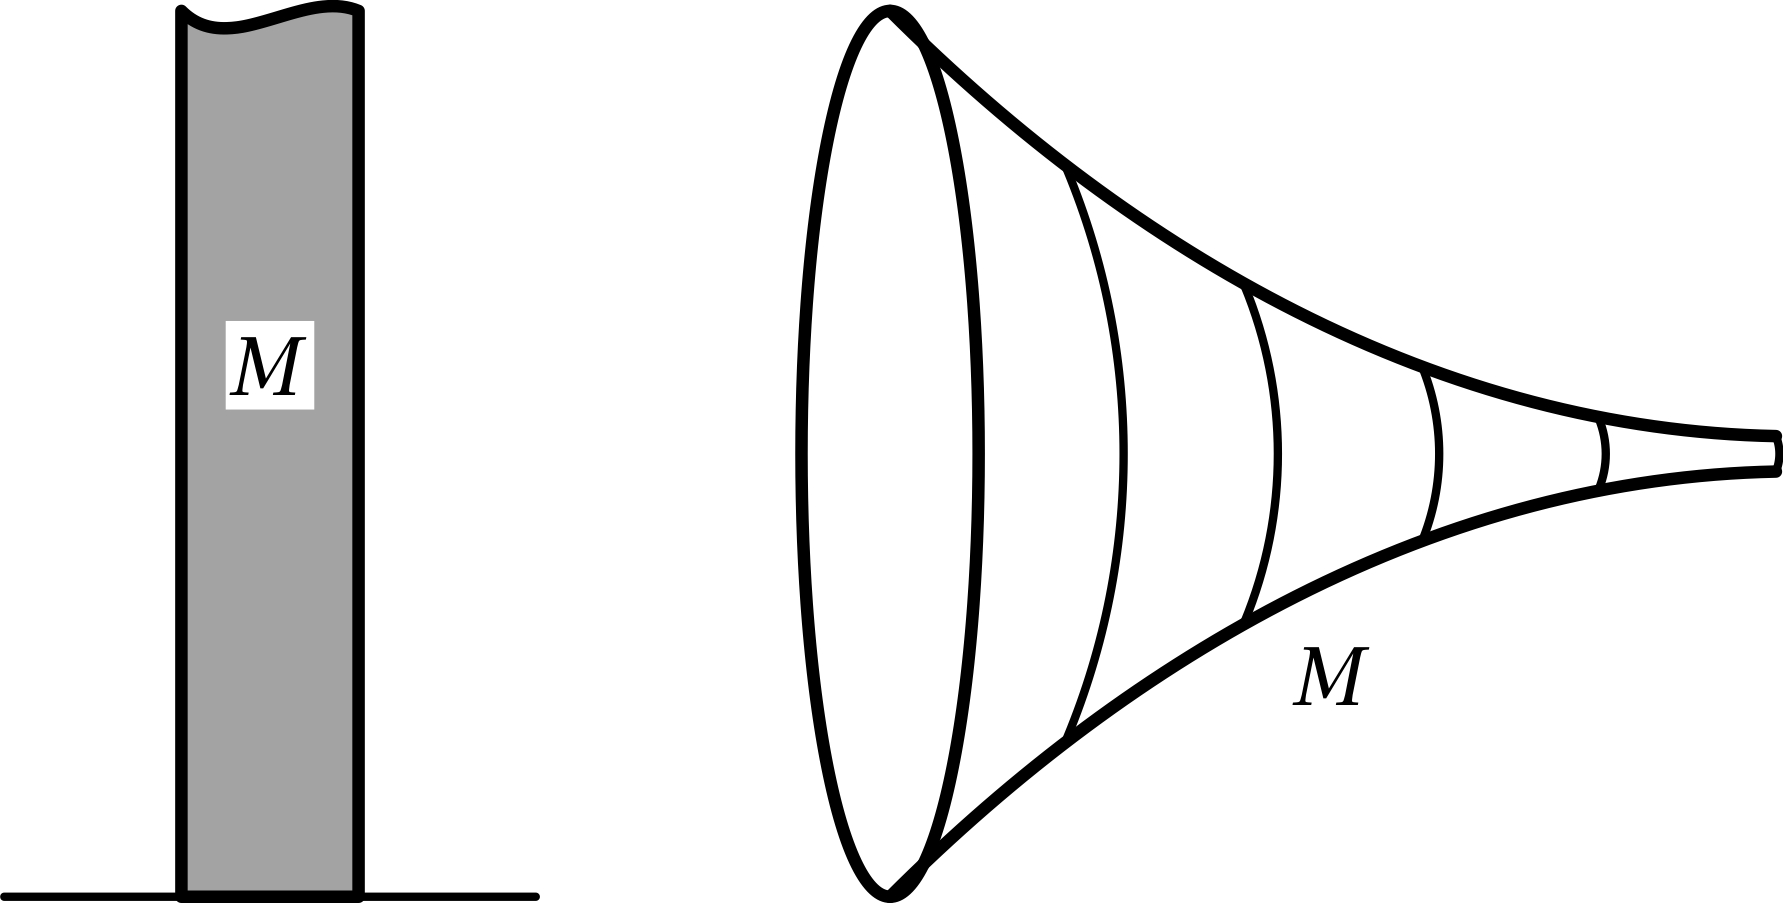
\includegraphics{PDF/M=cusp.jpg}$$
%texpreamble
%("  \usepackage{amsmath}
% \usepackage[LY1]{fontenc}
% \usepackage[expert,LY1,mylucidascale]{mylucidabr}
% ");
%defaultpen(  fontcommand("\normalfont") + fontsize(10) ); 
%
%from graph access *;
%unitsize(0.75cm);
%
%real linethick = 1.5;
%
%real w = 1, h = 5, M = 3, axis = 1;
%
%draw( (-axis,0)--(w + axis, 0), linewidth(1) );
%fill( (0,0)--(w,0)--(w,h){WNW}..{NW}(0,h)--cycle, gray(0.7) );
%draw( (0,0)--(w,0)--(w,h){WNW}..{NW}(0,h)--cycle, linewidth(linethick) );
%
%real bb = 0.25;
%fill( shift(w/2,M)*( (-bb,-bb)--(-bb,bb)--(bb,bb)--(bb,-bb) -- cycle), white);
%label( "$M$", (w/2,M) );
%
%
%currentpen = linewidth(linethick);
%
%real gap = 2, a = 5, b = 0.1, cusp;
%
%cusp = w + axis + gap;
%
%draw( (cusp,0){NE}..{(1,0.02)}(cusp + a,(h/2)-b) );
%draw( (cusp,h){SE}..{(1,-0.02)}(cusp + a,(h/2)+b) );
%draw( ellipse( (cusp,h/2), 0.5, h/2) ) ;
%
%currentpen = linewidth(1);
%
%//draw( (cusp, 0){NNW}..{NNE}(cusp, h) );
%//draw( (cusp, 0){NNE}..{NNW}(cusp, h) );
%draw( (cusp+(a/5), 0.9){NNE}..{NNW}(cusp+(a/5), h-0.9) );
%draw( (cusp+2*(a/5), 1.55){NNE}..{NNW}(cusp+2*(a/5), h-1.55) );
%draw( (cusp+3*(a/5), 2){NNE}..{NNW}(cusp+3*(a/5), h-2) );
%draw( (cusp+4*(a/5), 2.3){NNE}..{NNW}(cusp+4*(a/5), h-2.3) );
%draw( (cusp+5*(a/5), 2.4){NNE}..{NNW}(cusp+5*(a/5), h-2.4) );
%
%label( "$M$", (6.5,1.25) );

\begin{enumerate}

\item Any point far out in the cusp lies on a short loop that is not
null-homotopic, but points at the other end do not lie on such a
loop. Therefore, $M$ is not homogeneous, so it cannot be symmetric.

\item The geodesic symmetry performs a $180^\circ$ rotation. Therefore, if
it is a well-defined diffeomorphism of~$M$, it must
interchange the two ends of the cusp. However, one end is thin, and
the other end is (very!) wide, so no isometry can interchange these
two ends. Hence, the geodesic symmetry (at any point) is not an
isometry, so $M$ is not symmetric.

\item Let us show, directly, that the geodesic symmetry at some
point $p \in \hyperbolic^2$ does not factor through to a well-defined
map on $\Gamma \backslash \hyperbolic^2 = M$.

 \begin{itemize}
 \item Let $x = -1 + i$ and $y = 1+i$, and let $p \in i\real$ be the
midpoint of the geodesic segment joining~$x$ and~$y$:
%\begin{figure}[h]
$$ 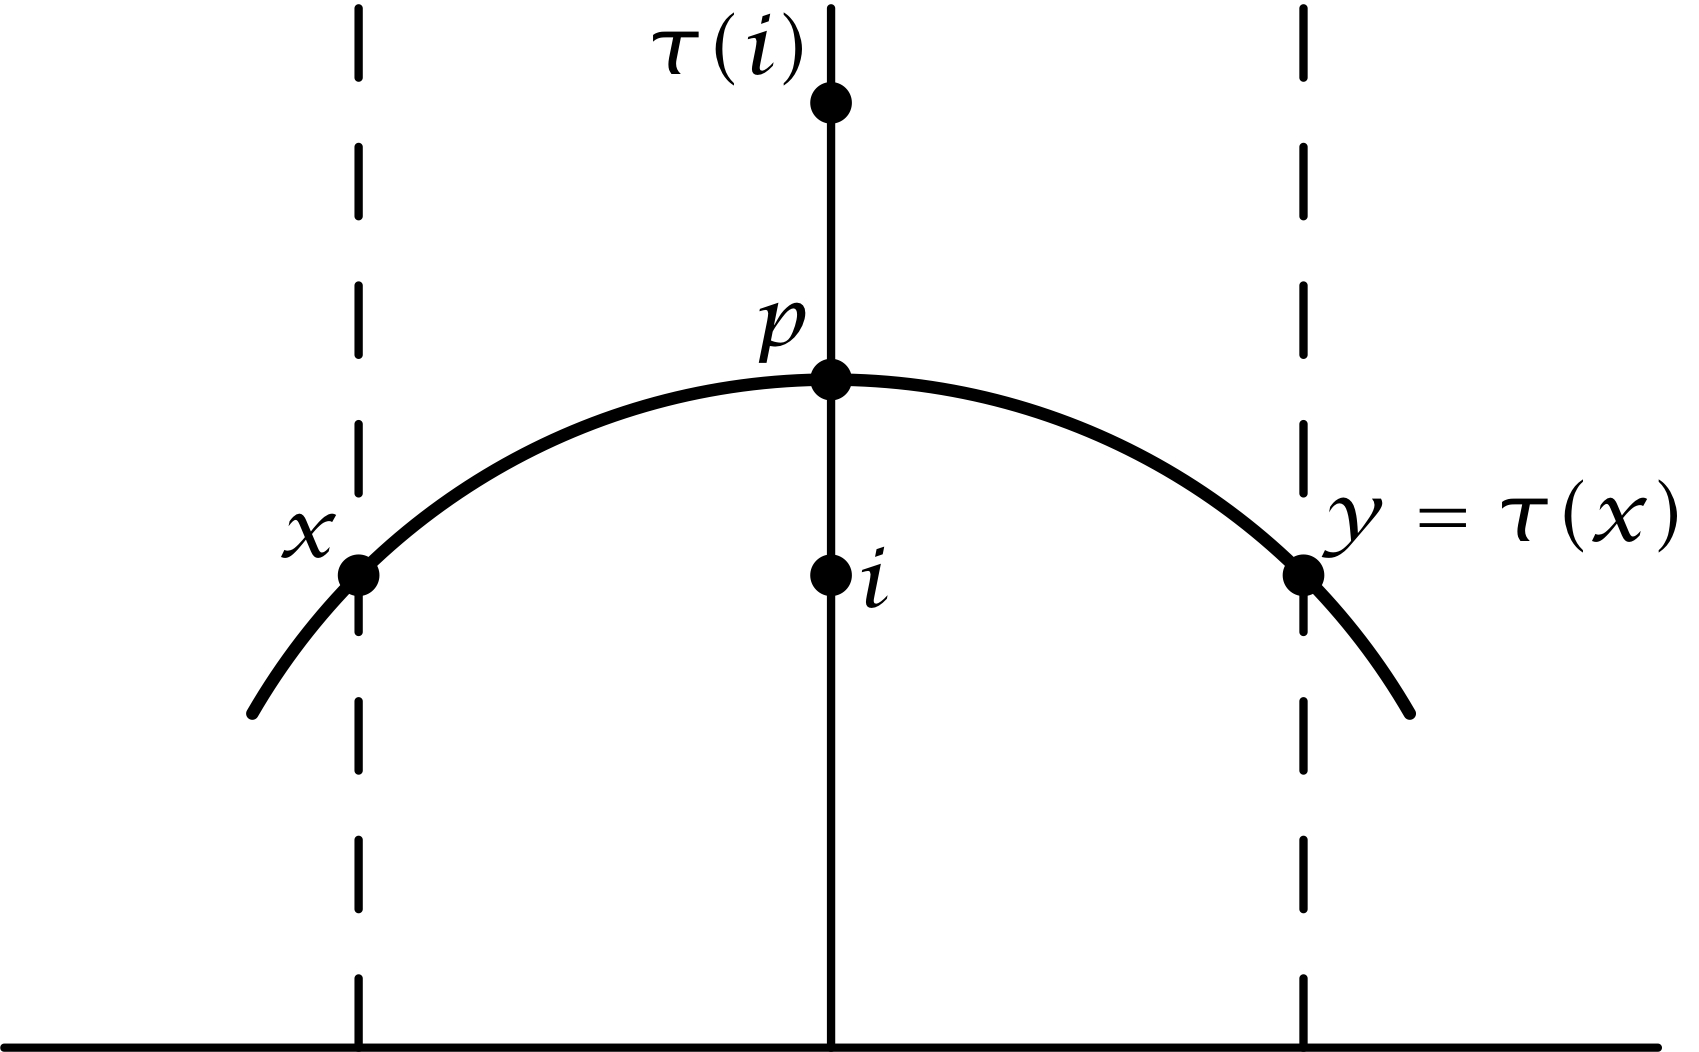
\includegraphics{PDF/CuspNotSymm.jpg} $$
% \caption{The geodesic symmetry~$\tau$ at~$p$.}
%\label{CuspNotSymm}
% \end{figure}
%texpreamble
%(" \usepackage[LY1]{fontenc}
% \usepackage[expert, LY1, mylucidascale]{mylucidabr} % I adjusted the scaling
% \usepackage{amsmath}
% ");
%defaultpen(  fontcommand("\normalfont") + fontsize(10) ); 
%
%from graph access *;
%unitsize(2cm);
%
%real r = sqrt(2), a = -1, b = 1;
%
%currentpen= defaultpen + linewidth(1.5);
%
%pair x = (a,b), y = (-a,b), p = (0,r), i = (0,1), ti = (0, 2) ;
%
%real w = 1.75*x.x, h = 1.1*ti.y;
%
%draw( (w,0)--(-w,0), linewidth(1) );
%draw( (0,0)--(0,h), linewidth(1) );
%
%draw( (x.x,0)--(x.x,h), dashed + linewidth(1) );
%draw( (y.x,0)--(y.x,h), dashed + linewidth(1) );
%
%label( "$x$" , x , NW);
%label( "$y = \tau(x)$" , y , NE);
%label( "$p$" , p , NW);
%label( "$i$" , i , E);
%label( "$\tau(i)$" , ti , NW);
%draw( x , linewidth(5) );
%draw( y , linewidth(5) );
%draw( p , linewidth(5) );
%draw( i , linewidth(5) );
%draw( ti , linewidth(5) );
%
%draw( arc( (0,0), r, 30, 150 ) );

 \item Let $\tau$ be the geodesic symmetry at~$p$. Then $\tau(x) = y
= 1 + i$.
 \item Because the imaginary axis is a geodesic, we have $\tau(i) =
ai$, for some $a > 1$.
 \item Now $i = x + 1 = g(x)$, so $x$ and~$i$ represent the same point
in~$M$. However, $\tau(i) - \tau(x) = -1 + (a-1)i$ is not an
integer (it is not even real), so $\tau(x)$ and~$\tau(i)$ do
\textbf{not} represent the same point in~$M$.  Therefore, $\tau$ does not
factor through to a well-defined map on~$M$.
 \end{itemize}

 \end{enumerate}
 \end{eg}

 \begin{rems} \ \label{locsymm<>curv}
 \noprelistbreak
 \begin{enumerate}
 \item Some authors do not require $M$ to be complete in their
definition of a locally symmetric space. This would allow the
universal cover of~$M$ to be an open subset of a symmetric space,
instead of the entire symmetric space.
 \item A more intrinsic (but more advanced) definition is that a
complete, connected Riemannian manifold~$M$ is \defit[locally!symmetric]{locally
symmetric} if and only if the curvature tensor of~$M$ is invariant
under all parallel translations, and $M$ is complete. 
 \end{enumerate}
 \end{rems}

Any complete, connected manifold of constant negative curvature is a
locally symmetric space, because the universal cover of such a manifold is $\hyperbolic^n$  (after normalizing the curvature to be~$-1$).
As a generalization of this, we are interested in locally symmetric
spaces~$M$ whose universal cover~$\widetilde{M}$ is of
\defit{noncompact type}, with no flat factors; that is, such that
each irreducible factor of $\widetilde{M}$ is noncompact (and not
flat).  From \cref{noncpctsymm<>simplegrp}, we see, in this
case, that $\widetilde{M}$ can be written in the form $\widetilde{M} = 
G/K$, where $G = G_1 \times \cdots \times G_n$ is a product of
noncompact simple Lie groups, and $K$~is a maximal compact subgroup
of~$G$. We have $M = \Gamma \backslash \widetilde{M}$, for some discrete subgroup~$\Gamma$ of $\Isom \bigl(  \widetilde{M}  \bigr)$. We know that $\Isom \bigl(  \widetilde{M} \bigr)$ has only finitely many connected components \csee{IsomFinComps}, so, if we replace $M$ with an appropriate finite cover, we can arrange that $\Gamma \subset \Isom \bigl( \, \widetilde{M} \, \bigr)^\circ = G$. Then
	$$ \text{$M = \Gamma \backslash G/K$, and $\Gamma$~is a discrete subgroup of~$G$.} $$

A topologist may like $M$ to be compact, but it turns out that a
very interesting theory is obtained by making the weaker assumption
that $M$ has finite volume. Hence, the subgroup~$\Gamma$ should be
chosen so that $\Gamma \backslash G/K$ has finite volume. Because
$\Gamma \backslash G$ is a principal $K$-bundle over $\Gamma
\backslash G/K$, and $K$~has finite measure, it is not difficult to
see, from \thmindex{Fubini's}{Fubini's Theorem}, that $\Gamma \backslash G$ has finite
volume \csee{lattice<>mu(X/Gamma)}. This leads to the following
definition.

\begin{defn}
 A subgroup~$\Gamma$ of~$G$ is a \defit[lattice!subgroup]{lattice} in~$G$ if $\Gamma$~is discrete and $\Gamma \backslash G$ has finite volume
\textup(which respect to the Haar measure on~$G$\textup). 
 \end{defn}

\begin{eg}
If $\Gamma$ is discrete and $\Gamma
\backslash G$ is compact, then $\Gamma$ is a lattice in~$G$, because
any compact Riemannian manifold obviously has finite volume.
\end{eg}

\begin{eg} \label{SL2Zlatt}
 $\SL(2,\integer)$ is a lattice in $\SL(2,\real)$. To see this, let
 \begin{equation} \label{SL2ZFundDom}
 \fund = \{\, z \in \hyperbolic^2 \mid \mbox{$|z|
\ge 1$ and $-1/2 \le \Re z \le 1/2$} \,\} 
 \end{equation}
 \csee{FundDomSL2R}. It is well known (though not obvious) that
$\fund$ is a fundamental domain for the action of $\SL(2,\integer)$
on~$\hyperbolic^2$ \csee{SL2ZinFundDom,SL2ZBdryFundDom}; it
therefore suffices to show that $\fund$ has finite volume, or, more
precisely, finite hyperbolic area. 

\begin{figure}[t]
 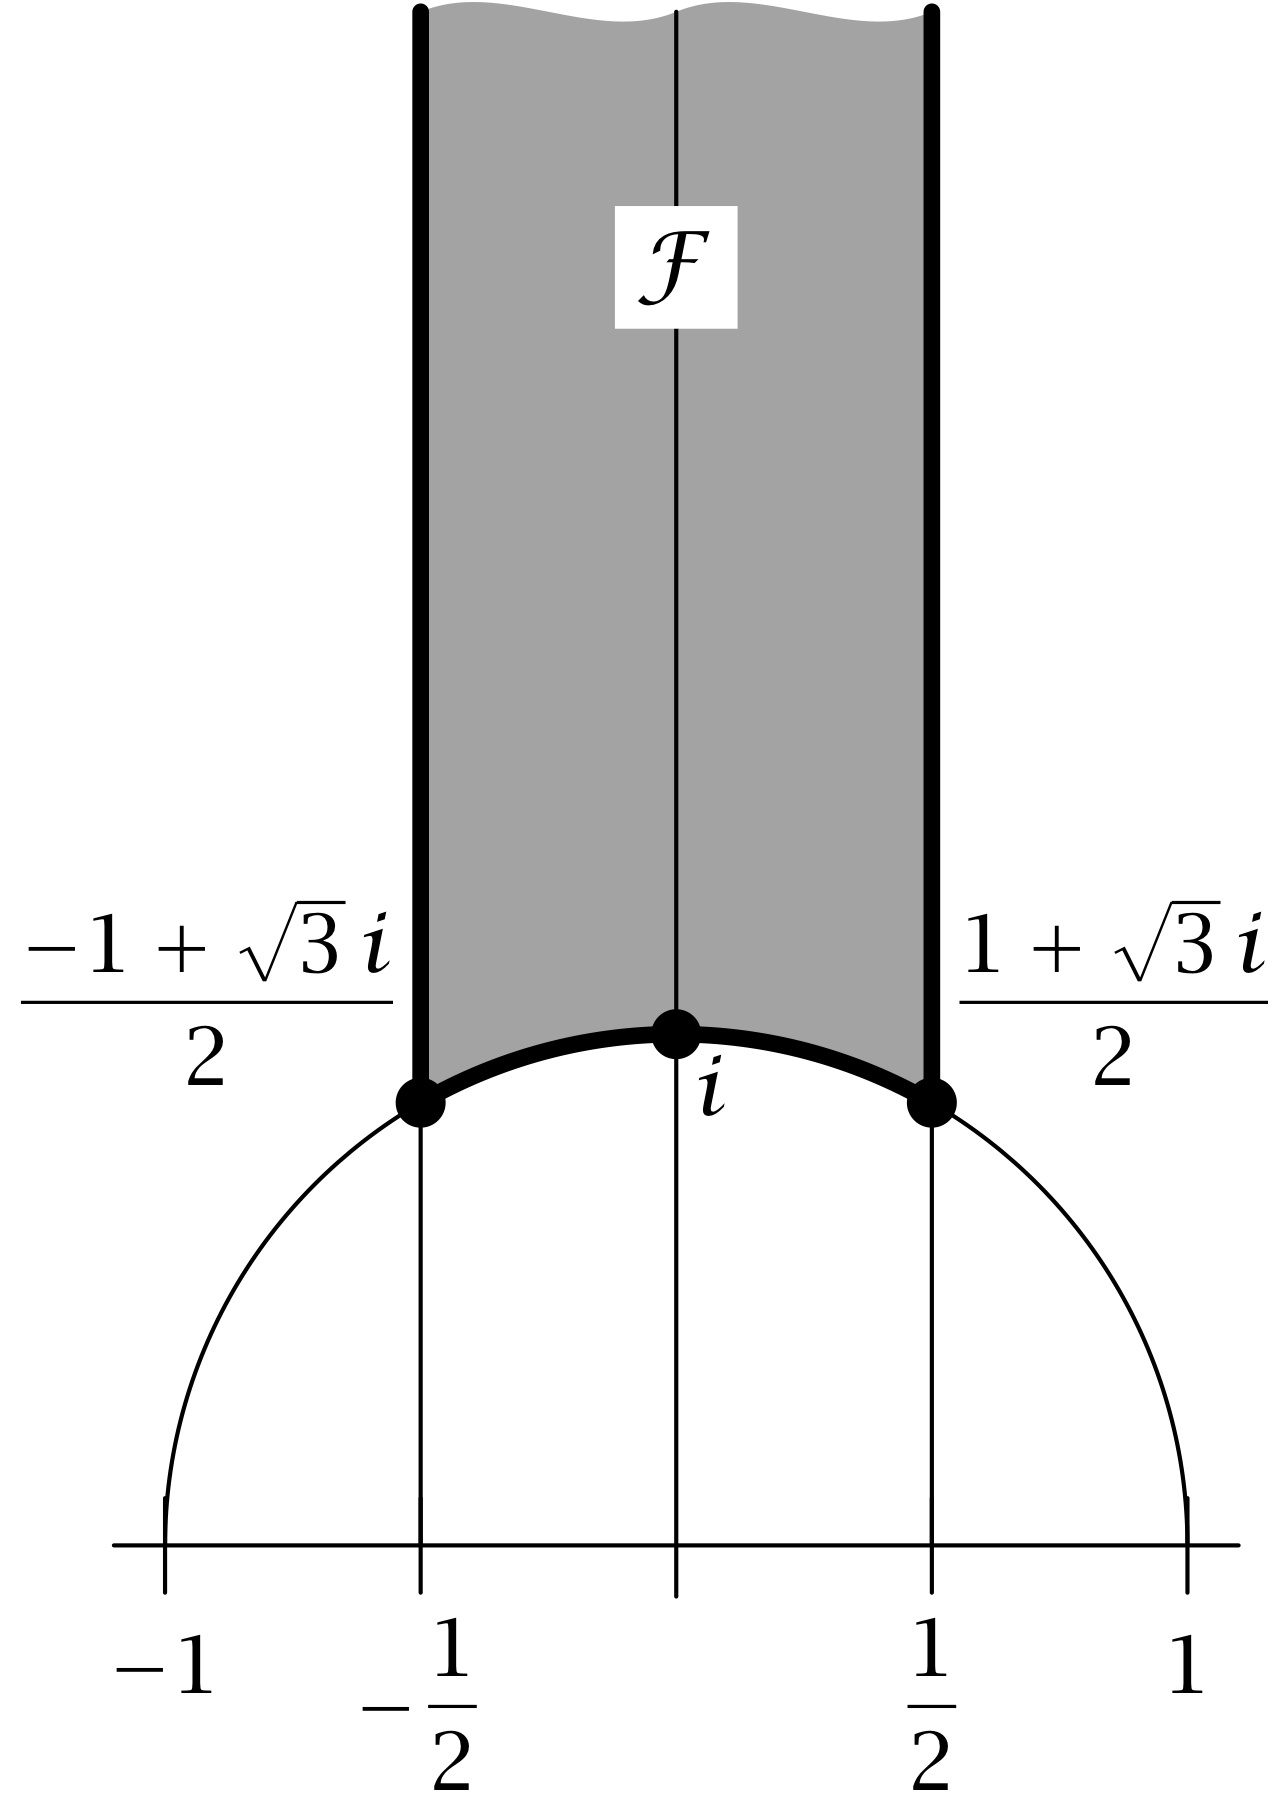
\includegraphics{PDF/FundDomSL2R.jpg}
 \caption{A fundamental domain~$\fund$ for $\SL(2,\integer)$ in
$\SL(2,\real)$.} \label{FundDomSL2R}
 \end{figure}
%texpreamble
%(" \usepackage[LY1]{fontenc}
% \usepackage[expert, LY1, mylucidascale]{mylucidabr} % I adjusted the scaling
% \usepackage{amsmath}
% \everymath{\displaystyle}
% ");
%defaultpen(  fontcommand("\normalfont") + fontsize(10) ); 
%
%from graph access *;
%
%size(0,3inch);
%pair i = (0,1);
%real h = sqrt(3)/2;
%pair a = (-1/2, h);
%pair b = (1/2, h);
%real top = 3;
%filldraw( (1/2,h) .. i .. (-1/2,h)--(-1/2,top){ENE}..{ENE}(0,top){ENE}..{ENE}(1/2,top)--cycle , gray(0.7) , invisible  );
%draw( (-1/2,h)--(-1/2,top) , linewidth(2) );
%draw( (1/2,h)--(1/2,top) , linewidth(2) );
%draw( (-1/2,h) .. i .. (1/2,h) , linewidth(2) );
%draw( (-1,0){N}..(-1/2,h) .. i .. (1/2,h) .. {S}(1,0));
%draw( (-1/2,0) -- (-1/2,h) );
%draw( (1/2,0) -- (1/2,h) );
%dotfactor = 12;
%dot( i ); label( "$i$", (0,1), SE );
%dot( a ); label( "$\frac{-1 + \sqrt{3} \, i}{2}$", a , NW );
%dot( b ); label( "$\frac{1 + \sqrt{3} \, i}{2}$", b , NE );
%real[] xticklist = {-1, -1/2, 1/2, 1};
%string labelfunc(real x){ 
%	if (x < -0.75){return "$-1$";} 
%	else if (x > 0.75) { return "$1$" ;}
%	else if (x < 0) { return "$-\frac{1}{2}$" ;}
%	else { return "$\frac{1}{2}$" ;}
%	}
%xaxis(-1.1, 1.1, Ticks(xticklist, ticklabel=labelfunc) );
%yaxis(-0.1, top, true);
%
%real fundw = 0.12, fundh = 2.5;
%fill( (-fundw, fundh - fundw) -- (fundw, fundh - fundw) -- (fundw, fundh + fundw) --  (-fundw, fundh + fundw) -- cycle, white );
%label( "$\mathcal{F}$",  (0,fundh) );

The hyperbolic area~$dA$ of an infinitesimal rectangle is the product
of its hyperbolic length and its hyperbolic width. If the Euclidean
length is $dx$ and the Euclidean width is $dy$, and the rectangle is
located at the point $x + iy$, then, by definition of the hyperbolic
metric, the hyperbolic length is $(dx)/(2y)$ and the hyperbolic width
is $(dy)/(2y)$. Therefore, 
 $$ dA = \frac{dx \, dy}{4 y^2} .$$
 Since $\Im z \ge \sqrt{3}/2$ for all $z \in \fund$,
we have
 $$ \vol(\fund)
 = \int_{x + iy \in \fund} \, dA
 \le \int_{\sqrt{3}/2}^\infty \int_{-1/2}^{1/2} \, \frac{dx \, dy}{4
y^2}
 =  \frac{1}{4} \int_{\sqrt{3}/2}^\infty \frac{1}{y^2} \, dy 
 < \infty .$$

Unfortunately, $\SL(2,\integer) \backslash \hyperbolic^2$ is not a
locally symmetric space, because $\SL(2,\integer)$ does not act
freely on~$\hyperbolic^2$ (so the quotient space is not a Riemannian
manifold). However, there are finite-index subgroups of
$\SL(2,\integer)$ that do act freely \ccf{torsionfree}, and these
provide interesting locally symmetric spaces.
 \end{eg}

Calculations similar to (but more complicated than)
\cref{SL2Zlatt} show:
 \begin{itemize}
 \item $\SL(n,\integer)$ is a lattice in $\SL(n,\real)$, and
 \item $\SO(p,q) \cap \SL(n,\integer)$ is a lattice in $\SO(p,q)$.
 \end{itemize}
 As in the example of $\SL(2,\integer) \backslash \hyperbolic^2$, the
hard part is to find a fundamental domain for $\Gamma \backslash G$
(or an appropriate approximation of a fundamental domain); then it is
not difficult to see that its volume is finite.
 These are special cases of the following general theorem, which
implies that every simple Lie group has a lattice.

\begin{thm}[{(\thmindex{arithmetic subgroups are lattices}{Arithmetic subgroups are lattices} \csee{arith->latt})}]
\label{Arith->Latt}
 Assume 
 \begin{itemize}
 \item $G = G_1 \times \cdots \times G_m$ is a product of simple Lie
groups,
 \item $G \subseteq \SL(\ell,\real)$, and 
 \item $G \cap \SL(\ell,\rational)$ is dense in~$G$.
 \end{itemize} Then $G_{\integer} = G \cap \SL(\ell,\integer)$ is a
lattice in~$G$.
 \end{thm}

Lattices constructed by taking the integer points of~$G$ in this way
are said to be \defit[arithmetic!subgroup]{arithmetic} \csee{ArithDefn}. (For most
simple Lie groups, these are the only lattices \csee{MargulisArith}.)
When $\ell$ is large, there is more than one way to embed $G$ in
$\SL(\ell,\real)$, and we will see that different embeddings can lead
to quite different intersections with $\SL(\ell,\integer)$. In particular, if $G$ is a noncompact, simple Lie group, then:
	\begin{itemize}
	\item By taking
an appropriate embedding of~$G$ in some $\SL(\ell,\real)$, we will
construct a lattice~$\Gamma$ in~$G$, such that $\Gamma \backslash G$ is \textbf{not} compact \csee{GHasNoncpctLatt}.
	\item By taking a different
embedding, we will construct a different lattice $\Gamma'$, such that
$\Gamma' \backslash G$ is compact \csee{GHasCpctLatt}.
	\end{itemize}

We will also see that algebraic properties of~$\Gamma$ influence the geometry of the corresponding locally symmetric space~$M$. 
In particular, the structure of~$\Gamma$ determines whether $M$ is compact or not.
(For example, the ``Godement Criterion'' \pref{GodementNoCpctFactor} implies that $M$~is compact if and only if every element of~$\Gamma$ is a diagonalizable matrix over~$\complex$.)
%More generally, we will see how group-theoretic
%properties of $\Gamma$ influence the large-scale structure of~$M$ \csee{LargeScaleSect}.
Much more generally, the following important theorem implies that
every geometric property of~$M$ is faithfully reflected in some
group-theoretic property of~$\Gamma$. 

\begin{thm}[(\thmindex{Mostow Rigidity}{Mostow Rigidity Theorem} \csee{MostowChap})] \label{MostowIrred}
 Let $M_1$ and $M_2$ be finite-volume locally symmetric spaces\/ \textup(not both $2$-dimensional\/\textup), such
that
 \begin{itemize}
 \item the universal covers of~$M_1$ and~$M_2$ are neither compact,
nor flat, nor reducible,
and
\item the volumes of $M_1$ and~$M_2$ are normalized\/ \textup(i.e., $\vol M_1 = \vol M_2 = 1$\textup).
 \end{itemize}
  If\/ $\pi_1(M_1) \iso \pi_1(M_2)$, then $M_1$ is isometric to~$M_2$.

 In fact, every homotopy equivalence is homotopic to an isometry.
 \end{thm}

The theorem implies that locally symmetric spaces
have no nontrivial deformations, which is why it is called a ``rigidity'' theorem:

\begin{cor}
Let $\{g_t\}$ be a continuous family of Riemannian metrics on a manifold~$M$ with\/ $\dim M > 2$, such that, for each~$t$:
	\begin{itemize}
	\item $(M,g_t)$ is a finite-volume locally symmetric space  whose universal cover is neither compact, nor flat, nor reducible,
	and
	\item $\vol(M,g_t) = 1$.
	\end{itemize}
Then $(M,g_t)$ is isometric to $(M,g_0)$, for every~$t$.
\end{cor}

\begin{defn}
 A locally symmetric space is \defit[irreducible!locally
symmetric space]{irreducible} if no \emph{finite} cover of~$M$ can be
written as a nontrivial cartesian product $M_1 \times M_2$.
 \end{defn}

 It is important to note that the universal cover of an irreducible
locally symmetric space need not be an irreducible symmetric space.
In other words, there can be lattices in $G_1 \times \cdots \times
G_n$ that are not of the form $\Gamma_1 \times \cdots \times
\Gamma_n$ \csee{SL(2Z[sqrt2])}. 

\begin{rem}
\Cref{MostowIrred} (and the corollary) can be generalized to the case where
only~$M_1$, rather than the universal cover of~$M_1$, is irreducible.
However, this requires the hypotheses to be strengthened: it
suffices to assume that no irreducible factor of~$M_1$ or~$M_2$ is
either compact or flat or $2$-dimensional. Furthermore, the conclusion needs to be weakened:
rather than simply multiplying by a single scalar to normalize
the volume, there can be a
different scalar on each irreducible factor of the universal cover.
\end{rem}

\begin{exercises}

\item
 Let
 \begin{itemize}
 \item $X$ be a simply connected symmetric space, 
 \item $\Gamma \backslash X$ be a locally symmetric space whose
universal cover is~$X$ (so $\Gamma$ is a discrete group of isometries
that acts freely and properly discontinuously on~$X$), and
 \item $\tau$ be an isometry of~$X$.
 \end{itemize}
 Show that if $\tau$ factors through to a well-defined map on $\Gamma
\backslash X$, then $\tau$ normalizes~$\Gamma$ (that is, $\tau
\gamma \tau^{-1} \in \Gamma$, for every $\gamma \in \Gamma\mk$).

\item \label{GrpCuspNotSymm}
 Define $g \colon \hyperbolic^2 \to \hyperbolic^2$ by $g(z) = z+1$. 
 \begin{enumerate}
 \item Show the geodesic symmetry~$\tau$ at~$i$ is given by
$\tau(z) = -1/z$.
 \item Show that $\tau$ does not normalize $\langle g \rangle$.
 \item Conclude that $\tau$ does not factor through to a well-defined
map on $\langle g \rangle \backslash \hyperbolic^2$.
 \end{enumerate}

\item
 Let
 \begin{itemize}
 \item $X$ be a simply connected symmetric space, and
 \item $\Gamma \backslash X$ be a locally symmetric space whose
universal cover is~$X$ (so $\Gamma$ is a discrete group of isometries
that acts freely and properly discontinuously on~$X$).
 \end{itemize}
 Show that $X$ is homogeneous if and only if the normalizer
$\nzer_G(\Gamma)$ is transitive on~$X$, where $G = \Isom(X)$.

\item Let $M = \Gamma \backslash G/K$ be a locally symmetric space,
and assume that $G$ has no compact factors. Show that if
$\nzer_G(\Gamma)/\Gamma$ is finite, then $\Isom(M)$ is finite.

\item Show that if $K$ is any compact subgroup of a Lie group~$G$,
then there is a unique (up to a scalar multiple) $G$-invariant Borel
measure~$\nu$ on $G/K$, such that $\nu(C) < \infty$, for every
compact subset~$C$ of $G/K$.

\item \label{lattice<>mu(X/Gamma)}
 Let
\begin{itemize}
 \item $K$ be a compact subgroup of a Lie group~$G$, and
 \item $\Gamma$ be a discrete subgroup of~$G$ that acts freely on
$G/K$.
 \end{itemize}
 Show that $\Gamma \backslash G$ has finite volume if and only if
$\Gamma \backslash G/K$ has finite volume.

\item \label{SL2ZinFundDom}
 Let $\Gamma = \SL(2,\integer)$, and define $\mathcal{F} \subset
\hyperbolic^2$ as in~\eqref{SL2ZFundDom}. Show, for each $p \in
\hyperbolic^2$, that there is some $\gamma \in \Gamma$ with
$\gamma(p) \in \mathcal{F}$.
 \hint{If $\Im \gamma(p) \le \Im p$ for all $\gamma \in \Gamma$, and
$-1/2 \le \Re p \le 1/2$, then $p \in \mathcal{F}$.}

\item \label{SL2ZBdryFundDom}
 Let $\Gamma = \SL(2,\integer)$, and define $\mathcal{F} \subset
\hyperbolic^2$ as in~\eqref{SL2ZFundDom}. Show, for $z,w \in
\mathcal{F}$, that if there exists $\gamma \in \Gamma$ with
$\gamma(z) = w$, then either $z = w$ or $z,w \in \bdry \mathcal{F}$.
 \hint{Assume $\Im w \le z$. Then $|\gamma_{2,1}z + \gamma_{2,2}| \le
1$. Hence $|\gamma_{2,1}| \in \{0,1\}$. If $|\gamma_{2,1}| = 1$ and
$\gamma_{2,2} \neq 0$, then $|\Re z| = 1/2$, so $z \in \bdry
\mathcal{F}$. If $|\gamma_{2,1}| = 1$ and
$\gamma_{2,2} = 0$, then $w = (az-1)/z$. Since $|\Re(1/z)|
\le |\Re z| \le 1/2$, and $|\Re w| \le 1/2$, we see that either $\Re
z = 1/2$ or $w = -1/z$.}

 \end{exercises}



\begin{notes}

 Either of Helgason's books \cite{HelgasonBookOld, HelgasonBook} is a
good reference for the geometric material on symmetric spaces and
locally symmetric spaces, the connection with simple Lie groups, and
much more. Lattices are the main topic of Raghunathan's book
\cite{RaghunathanBook}. 

\Cref{Arith->Latt} is a result of Borel and Harish-Chandra
\cite{BorelHarishChandra} that will be proved in \cref{SLnZLattChap,ReductionChap}.

\Cref{MostowIrred} combines work of Mostow
\cite{MostowRig}, Prasad \cite{PrasadRig}, and Margulis
\cite{Margulis-DiscGrpMot}. We will discuss it in  \cref{MostowChap}.

\Cref{SL2Zlatt} appears in many number theory texts, including \cite[\S7.1.2, pp.~77--79]{Serre-CourseArith}. Our hints
for \cref{SL2ZinFundDom,SL2ZBdryFundDom} are taken
from \cite[Prop.~4.4, pp.~181--182]{PlatonovRapinchukBook}.

\end{notes}



\begin{references}{9}

\bibitem{BorelHarishChandra}
 A.\,Borel and Harish-Chandra:
 Arithmetic subgroups of algebraic groups,
\emph{Ann. Math.} (2) 75 (1962) 485--535.
 \MR{0147566},
 \maynewline
 \url{http://dx.doi.org/10.2307/1970210}


\bibitem{HelgasonBookOld}
 S.\,Helgason:
 \emph{Differential Geometry and Symmetric Spaces.}
 American Mathematical Society, Providence, RI, 1962. 
   ISBN 0-8218-2735-9,
  \MR{1834454}

\bibitem{HelgasonBook}
 S.\,Helgason:
 \emph{Differential Geometry, Lie Groups, and Symmetric Spaces.}
 Academic Press, New York, 1978.
 \MR{0514561}

\bibitem{Margulis-DiscGrpMot}
 G.\,A.\,Margulis: 
 Discrete groups of motions of manifolds of non-positive curvature,
 \emph{Amer. Math. Soc. Translations} 109 (1977) 33--45.
 \MR{0492072}

\bibitem{MostowRig}
 G.\,D.\,Mostow:
 \emph{Strong Rigidity of Locally Symmetric Spaces.}
 Princeton Univ. Press, Princeton, 1973.
 \MR{0385004}

\bibitem{PlatonovRapinchukBook}
 V.\,Platonov and A.\,Rapinchuk: 
 \emph{Algebraic Groups and Number Theory.}
 Academic Press, Boston, 1994.
 ISBN 0-12-558180-7,
 \MR{1278263}

\bibitem{PrasadRig}
 G.\,Prasad:
 Strong rigidity of $\rational$-rank $1$ lattices,
 \emph{Invent. Math.} 21 (1973) 255--286. 
 \MR{0385005},
 \maynewline
 \url{http://eudml.org/doc/142232}
% \url{http://www.digizeitschriften.de/dms/resolveppn/?PPN=GDZPPN002090694}
% \url{http://dx.doi.org/10.1007/BF01418789}

\bibitem{RaghunathanBook}
 M.\,S.\,Raghunathan: 
 \emph{Discrete Subgroups of Lie Groups.}
 Springer, {New York}, 1972.
 ISBN 0-387-05749-8,
\MR{0507234}

\bibitem{Serre-CourseArith}
 J.--P.\,Serre:
 \emph{A Course in Arithmetic,}
 Springer, New York 1973.
 \MR{0344216}

 \end{references}


